\chapter{Umsetzung}
\section{Systemvoraussetzungen}
Für die Umsetzung unseres Vorhabens benötigen wir Python, um mit Django arbeiten zu können. Außerdem werden einige Pakete benötigt, die uns bei der Programmierung behilflich waren.

\section{Aufbau des Backend}
\label{Backend}
Zunächst musste ein Crawler geschrieben werden, der die entsprechenden Webseiten herunterlädt und abspeichert. Diesen Schritt haben wir mit Hilfe von Java umgesetzt. \newline

Da es den Anschein hatte, dass der Server den Zugriff nach ca. 100 Dokumenten verweigert, wurde der Crawler um eine Funktion erweitert, mit deren Hilfe man einen Webproxy zwischenschalten kann, der dieses Problem löst. Sobald ein Dokument nicht heruntergeladen werden kann, wird der nächste Proxy aus der Liste genommen. Die Proxy-Liste stammt von http://proxylist.hidemyass.com/ \cite{HMA2015}. Insgesamt wurden 7854 Dokumente heruntergeladen.\\

Im nächsten Schritt wurde ein Perl-Skript geschrieben, welches die vorhandenen Informationen extrahiert und in eine PostgreSQL Datenbank importiert. Hierfür wurde vorher ein entsprechendes Schema, welches in der folgenden Abbildung \ref{fig:ER-Diagramm} dargestellt ist, erstellt. Das Schema spiegelt die Informationen wider, die extrahiert und für den Import in die Datenbank normalisiert wurden. Hierzu zählen beispielsweise Informationen wie Geburtstag, Geburtsort, Größe und Links-/Rechtshänder.

\begin{figure}[H]
\centering
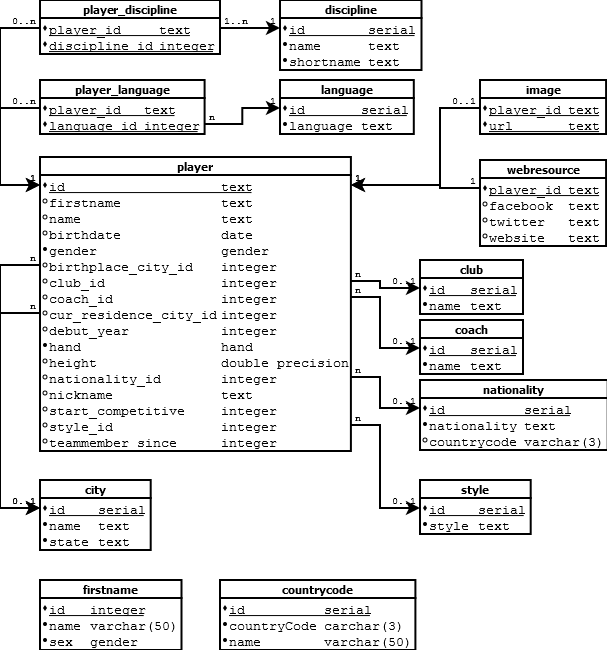
\includegraphics[width=1\textwidth]{images/ER-Diagramm} 
\caption{ER-Diagramm}
\label{fig:ER-Diagramm}
\end{figure}
\newpage

\section{Aufbau des Frontend}
\label{Frontend}
Die erstellte Webseite soll gut lesbar, schnell zu laden und intuitiv zu bedienen sein. Dafür wurde auf der Startseite ein kleines Navigationsmenü zur Unterteilung der einzelnen Features eingerichtet. \newline

Auf der Startseite erhält man einen kleinen Begrüßungstext, der das Ziel und die Funktionen der Webseite kurz beschreibt. Mit dem Suchformular ist es möglich, nach Spielern zu suchen, die gewisse Bedingungen erfüllen. Klickt man auf die etwas längliche Spieler-Id, werden alle wichtigen Informationen und, wenn vorhanden ein Bild des Spielers, angezeigt. Hier ist es auch möglich bestimmte Informationen für den Spieler zu setzen, wenn diese noch "`NULL"' sind. Sucht man beispielsweise nach dem deutschen Badmintonspieler Marc Zwiebler, ist es nur möglich den Verein einzutragen, da alle anderen Werte bereits gesetzt sind und viele Werte wie Geburtstag, Name und Geschlecht sich im Laufe des Lebens nicht ändern. \newline

Außerdem gibt es eine Reihe von vordefinierten Statistiken, die auf Basis der Datenbank erstellt wurden. Hierzu zählen:
Links- vs. Rechtshänder, Verein, Coach, Disziplin, Geschlecht, gesprochene Sprache/Muttersprache, aktuelle Nationalität und die Körpergröße. Zu guter Letzt gibt es einen Editor, mit dem Nutzer SQL-Anfragen schreiben können, um ihre eigenen Informationsbedürfnisse zu stillen.